


\begin{figure}[H]
    \centering
    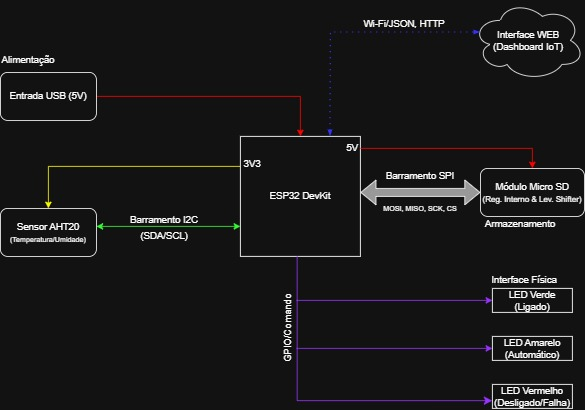
\includegraphics[width=\textwidth]{LaTeX/img_arquivo/DiagramaDeBlocos.png}
    
    \caption{Diagrama de Blocos do Sistema de Monitoramento de temperatura e umidade em ESP32 DevKit}
    \label{fig:diagramaDeBlocos}
\end{figure}

\subsection*{Descrição do Diagrama}

O diagrama ilustra a arquitetura completa do sistema de monitoramento de temperaturae umidade do ambiente. O núcleo é o ESP32 DevKit, que recebe alimentação de 5V via USB e distribui internamente a referência de 3,3V para os periféricos. O Sensor AHT20 (temperatura e umidade) comunica-se com o ESP32 pelo barramento I²C (SDA/SCL). Os dados são armazenados localmente em um Módulo Micro SD via barramento SPI (MOSI, MISO, SCK, CS), que possui um level shifter integrado para adequação dos níveis de tensão. O ESP32 também publica as leituras em um Dashboard IoT acessível remotamente por Wi-Fi, utilizando protocolo HTTP com payload em JSON. Por fim, três LEDs controlados por GPIO indicam o estado operacional: verde (ligado), amarelo (automático) e vermelho (desligado/falha).
